\documentclass[sigconf,authorversion,nonacm]{acmart}

\usepackage{float}
\usepackage{multirow}

\begin{document}

\title{UnVeilify: A Path Towards Personalized Face Mask Removal}

\author{Jin Hyoung Joo}
\email{hyoungjoo.j@gmail.com}
\affiliation{%
    \institution{Sungkyunkwan University}
    \country{Republic of South Korea}
}

\author{Minji Kim}
\email{kmjj7864@g.skku.edu}
\affiliation{%
    \institution{Sungkyunkwan University}
    \country{Republic of South Korea}
}

\author{Seungmin Lee}
\email{lsmbest@g.skku.edu}
\affiliation{%
    \institution{Sungkyunkwan University}
    \country{Republic of South Korea}
}

\author{Hyeonmin Lee}
\email{hyuni7185@g.skku.edu }
\affiliation{%
    \institution{Sungkyunkwan University}
    \country{Republic of South Korea}
}

\author{Hohyun Na}
\email{skghgus9@g.skku.edu}
\affiliation{%
    \institution{Sungkyunkwan University}
    \country{Republic of South Korea}
}

\author{Jaemin You}
\email{yjm7455@g.skku.edu}
\affiliation{%
    \institution{Sungkyunkwan University}
    \country{Republic of South Korea}
}

\begin{abstract}
    Our project aims to remove face masks from masked images while retaining the features
    of the target identity. Previous methods of removing facial masks exist,
    however do not consider the importance of identity preservation. We introduce
    a novel neural network architecture that combines the U-Net architecture with
    the StyleGAN generator to achieve this goal. We experimentally show that our method
    out-performs the previous methods in both quality and speed. Our code can be found at
    \url{https://github.com/jinhyoungjoo/UnVeilify}
\end{abstract}

\maketitle

\section{Introduction}
As the field of image generation is improving,
personalized image generation has drawn attention to many researchers, and as a
result, many astounding works have been done on this topic \cite{InstantBooth, SubjectDiffusion}.
However, most facial inpainting or facial reconstruction methods that attempt to encode the identity information \cite{SymmFC, IPFC, RGLSRI} all seem to
generate poor results and unusable quality for production. We belive this is due to the difficulty of successfully embedding the identity information to existing image generation frameworks.

In this paper, we introduce a specific task within the field of image inpainting.
We aim to remove facial masks from images, by proposing a novel neural network architecture.
Face masks have been, and will be part of many people's lives.
We believe that many people would like to remove this masks in images, since they view masks as occlusions rather than accesories.

This problem of removing face masks has also been dealt in other projects. Our project's
novelty comes in that these methods do not consider an important
aspect of the masked images, the identity features. Also, most of these projects show low quality image generation. Our model is capable of removing masks in a much higher quality within a very short time.

We first introduce other projects of mask removal and brief explanations of their methods. We then explain our approach to this task in much detail. Then we quantitatively and qualitatively analyze our approch, followed by our conclusion to this research.

\section{Related Work}
Previous methods of mask removal do exist. For example, \cite{GAN-Mask-Removal} approached
this problem by utilizing two separate networks. By first segmenting the mask regions from the
masked image, and inpainting the segmented region. \cite{STRV-ML} used a ResNet based U-Net architecture.
However, all these methods seem to either produce extremely low
quality results or disregard identity information and facial attributes entirely. This
results in image quality that is unusable in production (Figure \ref{images:bad_other}).

\begin{figure}
  \centering
  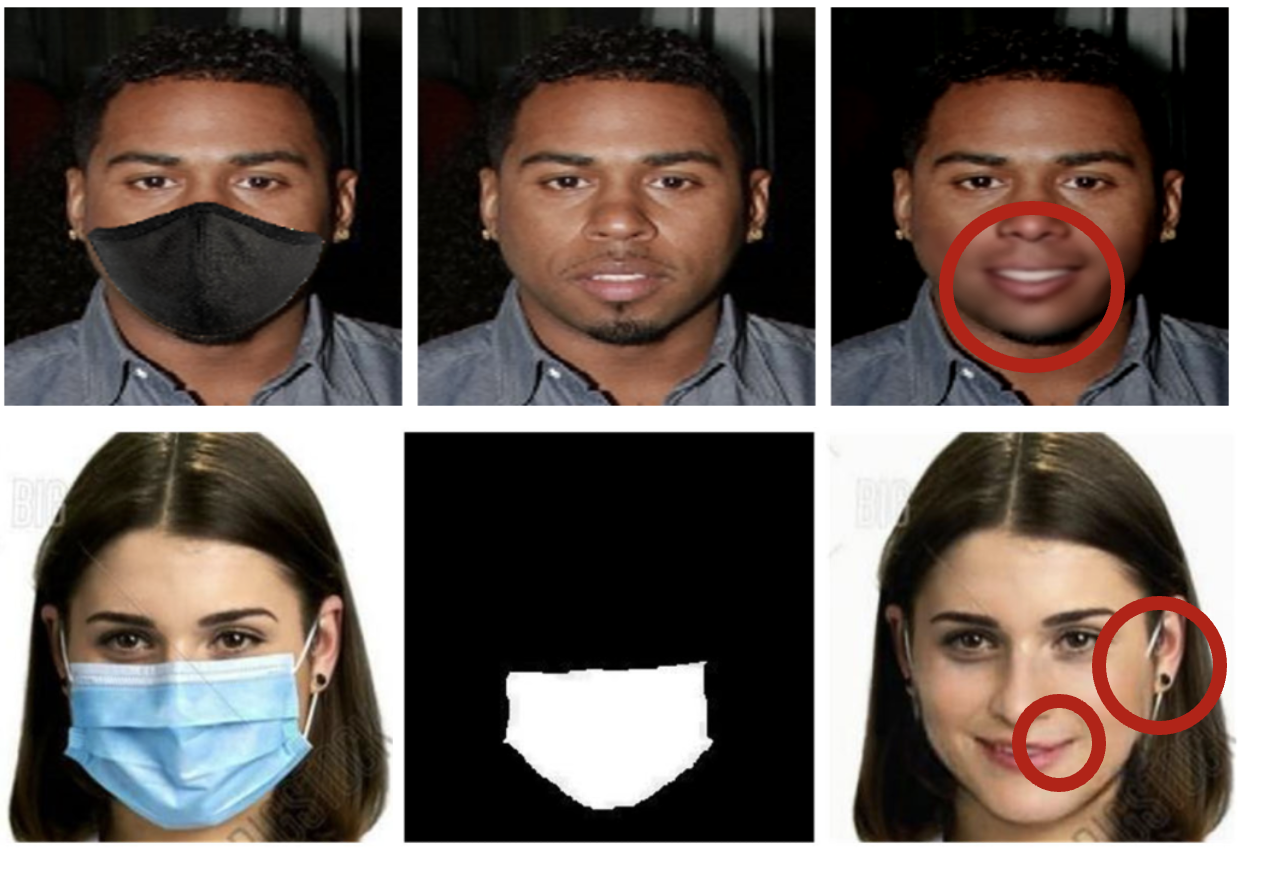
\includegraphics[width=\linewidth]{images/bad_other.png}
  \caption{\emph{Reported image results of other works.} The top image is the reported result of \cite{STRV-ML}. This does not consider the identity information and therefore looks like a different person compared to the ground truth. The bottom image is the reported result of \cite{GAN-Mask-Removal}. Since the ground truth is unreported, we could not evaluate the identity preservation of this image. However, it can be seen that artifacts exist that crucially degrades the quality of the image.}
  \Description{Overall architecture of the UnVeilify model.}
  \label{images:bad_other}
\end{figure}

\section{Method}
Our goal is to remove artifacts covering the facial area, namely face masks,
while preserving the identity of the original person behind the mask. This
requires us to generate the facial features by utilizing some sort of identity
information extracted from an image that contain no occlusions.

Therefore, we obtain two input images from the user, one as the image containing
the face mask to remove (we call this the \emph{masked image}) and the other as
the \emph{identity image} that shows the facial features of the identity the
user wishes to reconstruct. Here, the identity image isn't constrained to any
conditions, \emph{i.e.} the identity image and masked image are expected to be
independent in every way except for the identity of the person.

We first describe the overall architecture that we proposed. Next, each sub-module
of the network is described in detail. Finally, the objective functions used in our
research is explained.

\subsection{Overall Architecture}
Figure \ref{images:model-architecture} shows the overall architecture of the proposed network, named as \emph{UnVeilify}. The input
masked image goes through an encoder-decoder network, where the decoder is the StyleGAN generator
\cite{StyleGAN}. Although the architecture of this decoder is different in some ways from the
original StyleGAN model, to reduce confusion we leave the name as it is. Further description of this
updated generator architecture can be seen in the following sections.

The encoder consists of two main parts, the U-Net encoder that extracts the features from the masked image, and the PSP encoder that extracts the identity features from the identity image.

\begin{figure}
  \centering
  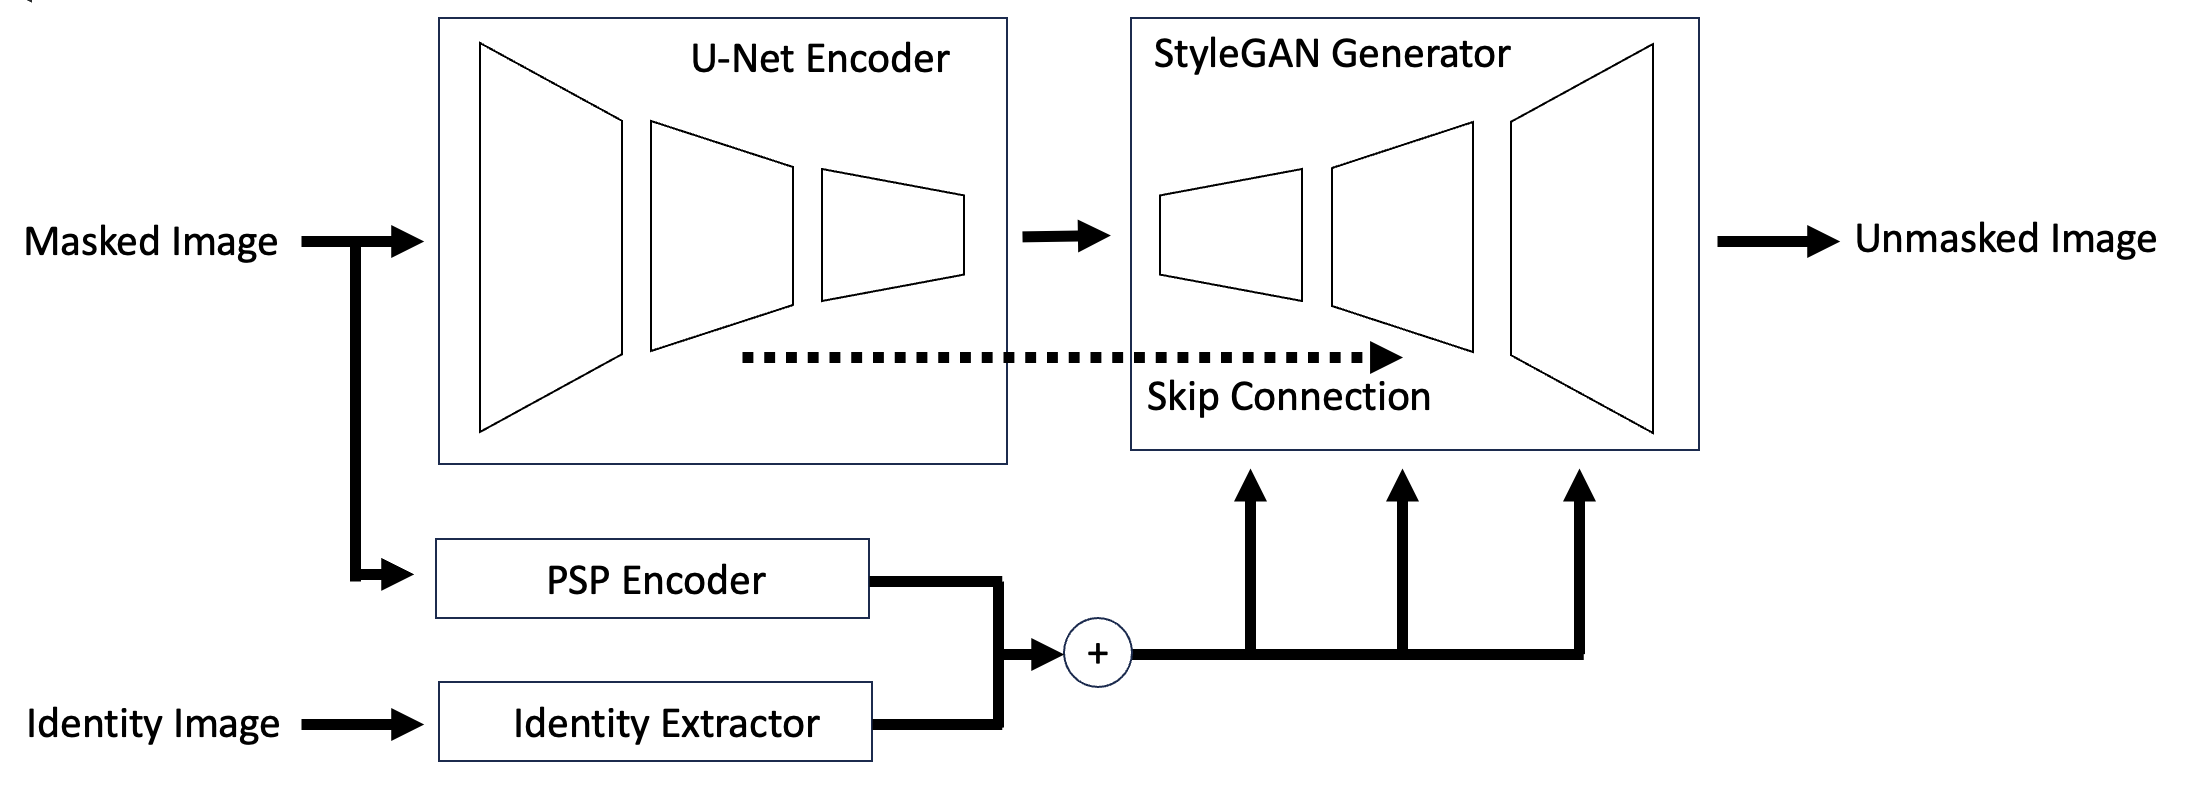
\includegraphics[width=0.8\linewidth]{images/model-architecture.png}
  \caption{\emph{Overall Architecture.} Our model consist of three main modules. The U-Net encoder extracts
  the features from the masked image. The PSP encoder extracts the features from the identity image. Finally,
the StyleGAN generator uses the extracted features to generate the unmasked image.}
  \Description{Overall architecture of the UnVeilify model.}
  \label{images:model-architecture}
\end{figure}

\subsection{Identity Extraction}
Our research began with attempting to implement the StyleGAN generator to our case. Since the
StyleGAN architecture is capable of producing high quality images while also providing controllable
styles via latent style vectors, we assumed that this type of architecture is exactly what we want.
However, while the StyleGAN architecture is capable of conditional image generation, it lacks the
ability for direct image-to-image translation. This is because finding the exact
latent style vectors to extract the features of the original domain is difficult.

The PSP encoder \cite{PSP} was introduced to address this problem. This encoder uses a ResNet backbone network to extract the features of an image to multiple style vectors that can be inserted in the StyleGAN generator in each layer.
By providing style guidance for low-level and high-level features, this encoder network can successfully generate images for image-to-image translation.

Our first approach to our task was to directly use this architecture. The PSP encoder does not change the StyleGAN architecture except for the generation of style vectors.
The authors explained that additional conditions can be inserted into the generator by adding or concatenating the vectors onto the style vectors. Our initial approach was to extract the image features from the masked image by this PSP encoder, and then add the identity vectors extracted from the identity image. This identity vector was the output of a pretrained face recognition network \cite{Arcface}.

However, we did not realize an important problem. While our task is an image-to-image translation, where the goal is to translate an image where the person is wearing a mask, to another domain where the person is not wearing the mask,
in this task the image features should remain exactly the same except for the mask region. Our initial approach does not consider this fact and by experimental results, generates very poor results.
Our solution to this problem was to use the PSP encoder as the style extractor from the identity image, and use a separate module that preserves the features of the original masked image. This module is the U-Net encoder and will be explained in the next section.

\begin{figure}[H]
  \centering
  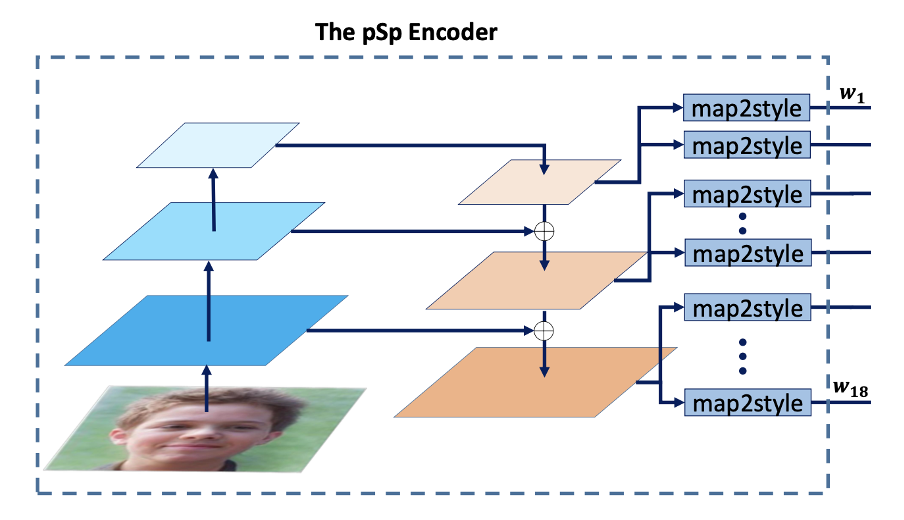
\includegraphics[width=0.8\linewidth]{images/psp-encoder.png}
  \caption{\emph{The PSP encoder.} The PSP encoder extracts information from a given image in multiple layers of information. This figure is taken from \cite{PSP}.}
  \Description{PSP encoder.}
\end{figure}

While there are other possibilites of extracting the identity information, we hypothesized
that the extraction of identity features is sufficiently done by the 
hierarchial feature pyramid network that extracts information from multiple different resolutions
of the image.

Also, while the authors of \cite{PSP} utilized a pretrained StyleGAN generator, due to our
novel network architecture where the original input image features are intact, there is no
need for any pretrained networks. This can help with further expandability to other domains,
especially where specialized datasets are difficult to obtain, since our network can train 
within a end-to-end setting with no pretrained networks.

\subsection{U-Net Encoder}
The U-Net encoder is based on the U-Net architecture \cite{UNet}. As mentioned above, the main
purpose of this encoder is to extract the features of the original masked image so that the final
generated image better preserves the information other than the masked region. The U-Net encoder
outputs skip connections and a downsampled image.

\begin{figure}[H]
  \centering
  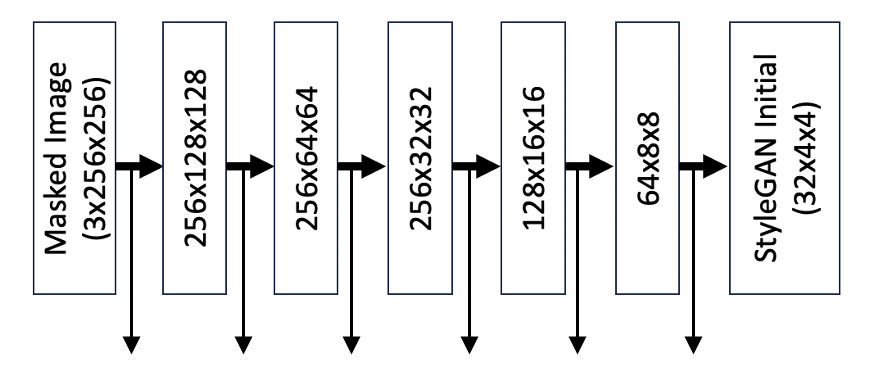
\includegraphics[width=0.8\linewidth]{images/unet.png}
  \caption{\emph{Detailed architecture of the U-Net encoder.}}
  \Description{PSP encoder.}
\end{figure}

First, the skip connections are inserted into the StyleGAN generator. This is different to the
original StyleGAN architecture, where additional vector inputs are not expected other than the
style vectors. We modified this by removing the single-channel noise inputs and instead use the multi-channel skip connections from the U-Net encoder.
The single-channel noise inputs in the original StyleGAN is used for generating stochastic detail, however we believed that this is unneccesary, since our task is not focused on diversity of the generated image, but rather has a ground truth image that it should match. 

The downsampled image outputted from the U-Net encoder is used as the initial starting point of the StyleGAN generator. This is different in that the original StyleGAN generator uses a constant learned parameter as the starting point. Also, the style vectors and skip connections are added to the
image channel-wise, where the weight of each vector is learned by the network. Our final model
adds these two vectors at almost the same weight, showing that for quality image generation, both
the style vector and skip connection are neccesary.
The final modified StyleGAN generator can be seen in Figure \ref{images:modified-stylegan}.

\begin{figure}
  \centering
  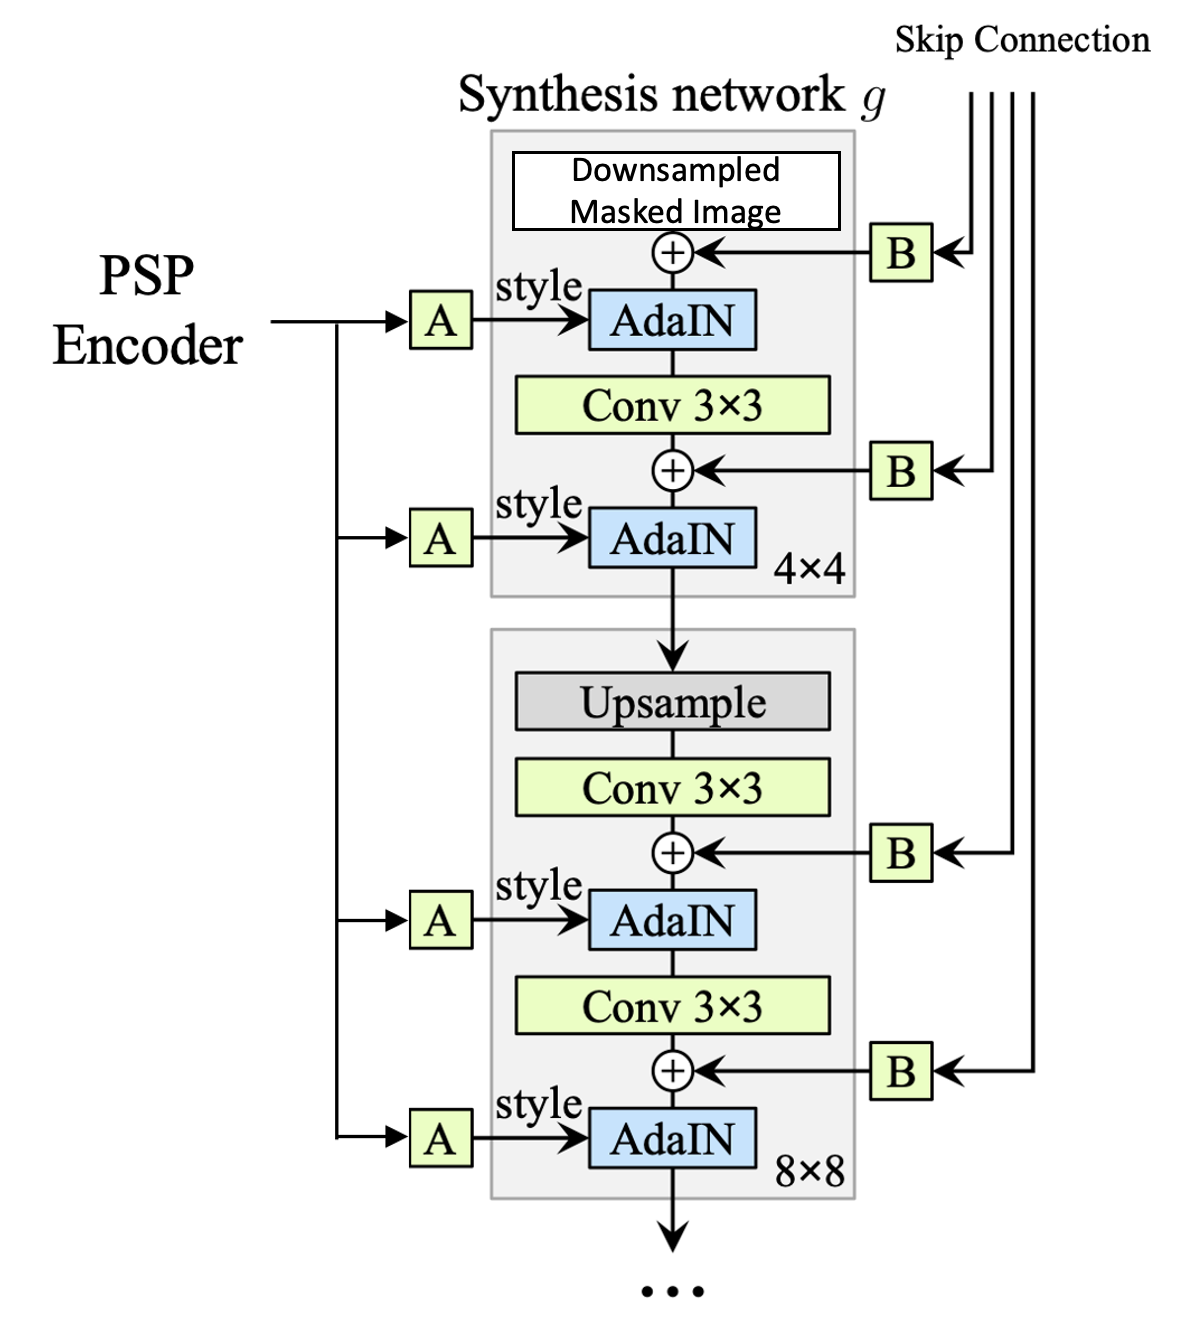
\includegraphics[width=0.8\linewidth]{images/modified-stylegan.png}
  \caption{\emph{The modified StyleGAN architecture.} Our modified StyleGAN generator utilizes the two input from the U-Net encoder and PSP encoder.}
  \Description{Modified StyleGAN architecture.}
  \label{images:modified-stylegan}
\end{figure}

\subsection{Objective Function}
Our models uses several loss functions to achieve the best quality possible. The final
objective function follows the form similar to the objective functions of other image-to-image
translation models.
We first use the $L1$ content loss in order to generate less blurry images
compared to that of using the $L2$ loss \cite{L1, Pix2Pix}. This loss is used as a
guide for generation by penalizing the distance between the ground truth unmasked image and
generated unmasked image.
\[
    L_{content}(\mathbf{y}, \mathbf{\hat{y}}) = \|\mathbf{y} - \mathbf{\hat{y}}\|_1
\]

We also use a perceptual loss in order to generate images with high visual qualities. We
utilize the LPIPS loss \cite{LPIPS} in the same way as \cite{PSP} has done,
since it has been shown that the LPIPS
loss preserves image quality better than other perceptual losses \cite{LPIPS2}.
\[
    L_{perceptual}(\mathbf{y}, \mathbf{\hat{y}}) = \|F(\mathbf{y}) - F(\mathbf{\hat{y}})\|_2
\]
Here, $F$ is the feature extractor used for the perceptual loss calculation.

This task focuses highly on identity preservation, where a large portion of the network
architecture design process is shifted towards this specific goal. Hence, in the objective
function we needed a method to also enforce identity preservation. This is achieved by
introducing an identity loss. By taking the cosine similiarity between the features of
a pretrained face recognition network (here we use ArcFace \cite{Arcface}), we can assume
that if the network trains to reduce this loss then the identity information loss would be
minimized.
\[
    L_{identity}(\mathbf{y}, \mathbf{\hat{y}}) = 1- C(R(\mathbf{y}) - R(\mathbf{\hat{y}}))
\]
Here, $R$ is the face recognition backbone model and $C$ is the cosine similiarity
function.

This model follows the form of a generative adversarial network, and incorporates a discriminator
and GAN loss. We use the objective function of the original GAN without any modifications.
However, since the identity image is given as a form of a conditional image, we give the
identity image paired with the unmasked image to the discriminator.
The discriminator is a simple PatchGAN \cite{PatchGAN} discriminator.
\[
    L_{GAN} (G, D) = \mathbb{E}_{y, c}\left[\log D(y, c)\right] + \mathbb{E}_{\hat{y}, c}\left[\log ( 1- D(\hat{y}, c))\right]
\]

The total objective function is the combination of these 4 separate objective functions.

\section{Experiments}
Our dataset requires a dataset of a masked image and an unmasked image that has everything except for the masked area to be the same. Since no dataset fits this criteria,
we use a synthesized dataset made from \cite{AI-Hub}, where the masked image is generated by
morphing face masks onto the detected facial landmarks. The final dataset consists of 8,746 masked and unmasked image pairs, with 31,604 identity images.
We use 80\% of the dataset as the training set and 10\% of the dataset as the test set and no
identities overlap between the training set and test set.

Also, due to the lack of properly working open-source code on mask removal, we set an image
inpainting model \cite{DMFN} as our baseline model. We train this baseline model on our dataset,
with the goal of generating the covered lower half of the masked image.
We use the following metrics as evaluation metrics. We also use metrics computed by \cite{GAN-Mask-Removal}.
These metrics are not evaluated on our test set, however can be used as one comparison criteria against other mask removal projects.

In order to evaluate the pixel-wise
difference between the ground truth and generated image, we incorporate the PSNR metric and
SSIM metric.
To compare the perceptual differences, we use the LPIPS metric \cite{LPIPS} that uses
a pretrained VGG network.

We trained our model on a single NVIDIA V100 GPU for 87 epochs. We used early stopping with the
validation set. Adam optimizers are used for both the generator and discriminator
with the learning rate set as 0.0002 for both models.

Our experimental results can be seen in Table \ref{table:experiment-results}. Our model performs
better in terms of PSNR, and although slightly performs lower in SSIM and LPIPS, we believe this
is because of the blurry results generated by the baseline model \cite{BadSSIM1, BadSSIM2}. This
can be seen in a qualitative analysis (Figure \ref{images:good-results}), our model generates
less blurry results compared to the baseline model and also generates images with identity information closer to the ground truth.

\begin{table*}[t]
\begin{tabular}{|l|l|l|l|l|}
\hline
 & PSNR & SSIM & LPIPS & Execution Time \\ \hline
Baseline Model (DMFN) \cite{DMFN} & 26.92 & \emph{0.90} & \emph{0.03} & 1404 ms  \\ \hline
Baseline Model (GAN-based Mask Removal) \cite{GAN-Mask-Removal} & 26.19 & 0.86 & Unreported & Unreported \\ \hline
UnVeilify (No U-Net Encoder) & 3.42 & 0.00 & 0.91 & 34 ms\\ \hline
UnVeilify (No Identity Image Given) & 6.57 & 0.01 & 0.89 & \multirow{3}{*}{55 ms} \\ \cline{1-4}
UnVeilify (Unnormalized Identity Features) & 19.16 & 0.75 & 0.14 & \\ \cline{1-4}
\emph{UnVeilify (Final Model)} & \emph{27.04} & 0.84 & 0.06 & \\ \hline
\end{tabular}
\caption{\emph{Experimental results of our model.}}
\label{table:experiment-results}
\end{table*}

\begin{figure}[ht]
  \centering
  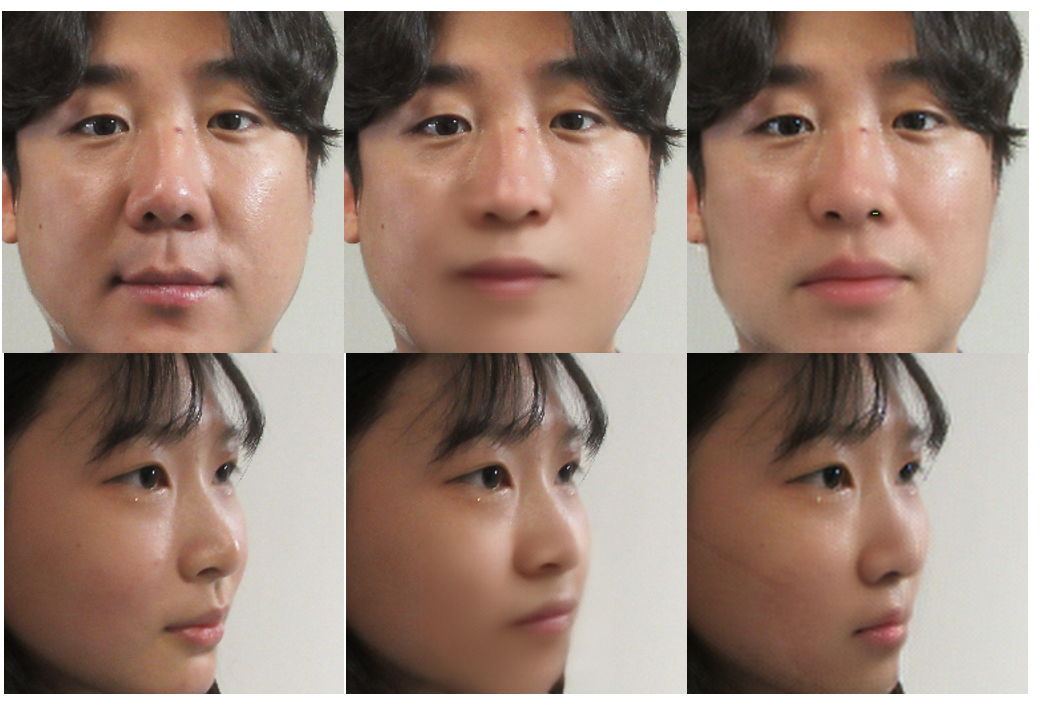
\includegraphics[width=0.8\linewidth]{images/good-results.png}
  \caption{\emph{Image results of our model compared to the baseline model.} Generated image 
  results from the test set. Starting from the left are from: the ground truth, the baseline model (DMFN), and our model (UnVeilify).}
  \Description{Image results}
  \label{images:good-results}
\end{figure}

Our model also out-performs the GAN-based mask removal method, showing that our method can generate more quality results compared to other mask removal methods. Our model can also generate images with highly less blurry results, which seem to be a common theme among all other mask removal methods.
\begin{figure}[ht]
  \centering
  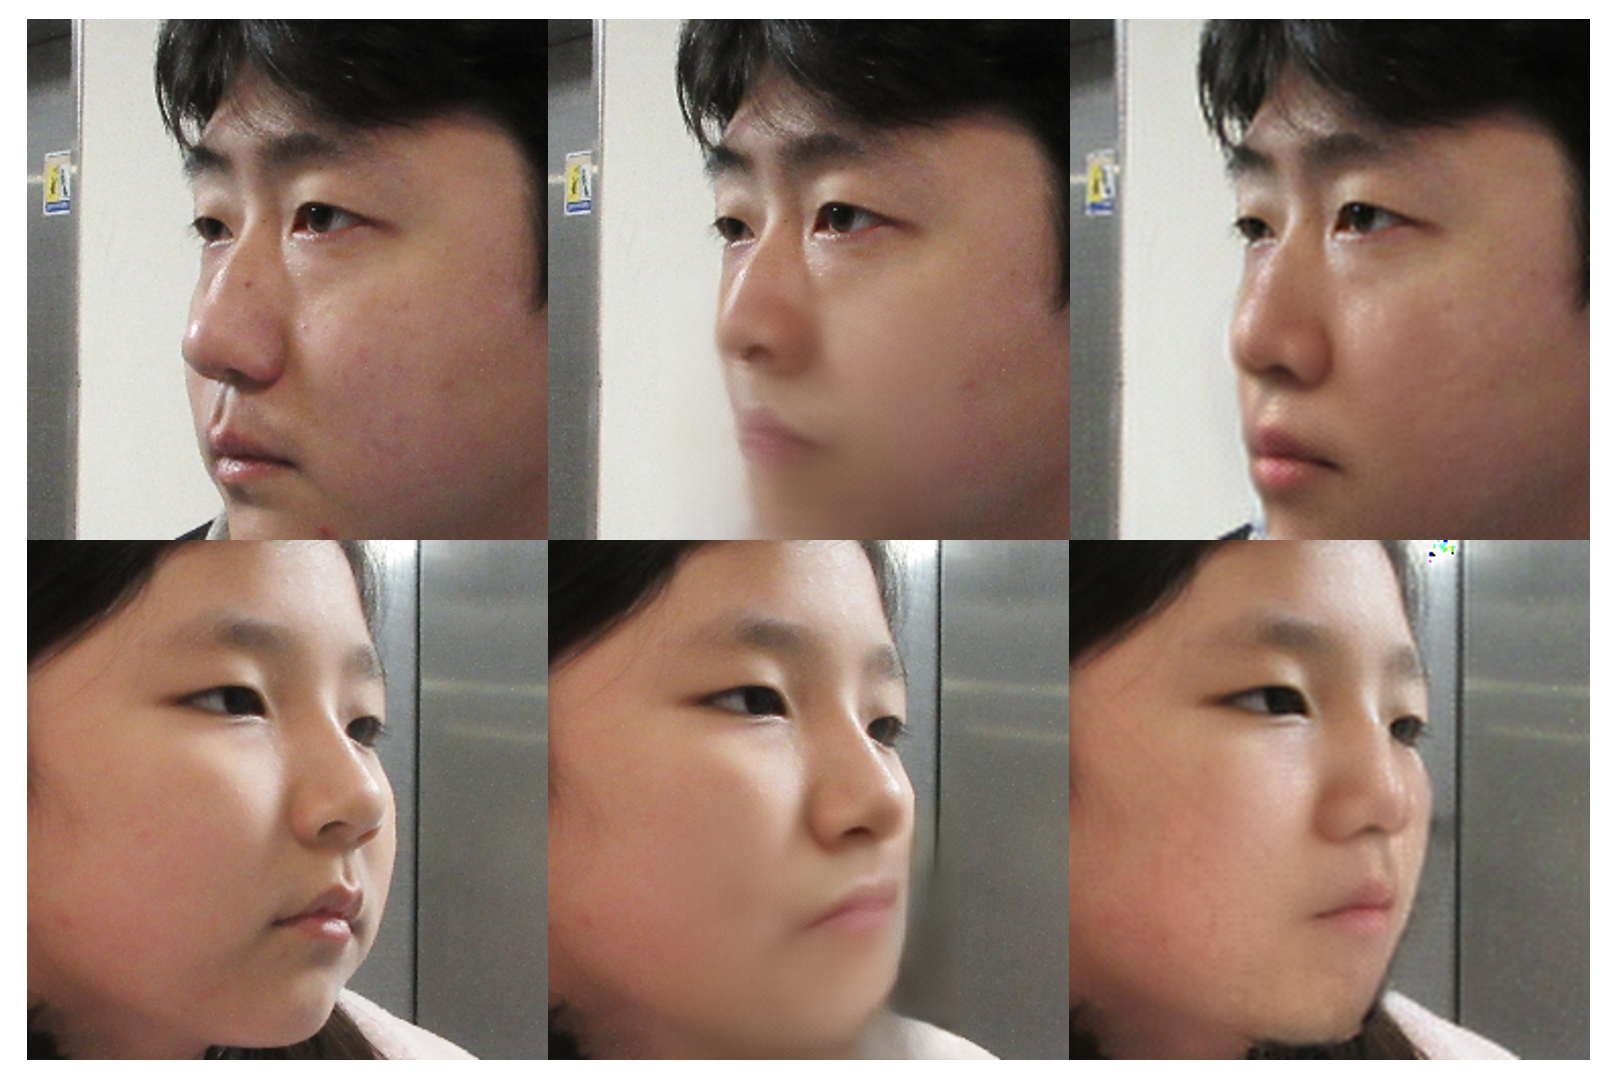
\includegraphics[width=0.8\linewidth]{images/bad-2.png}
  \caption{\emph{Image results of our model compared to the baseline model.} Generated image 
  results from the test set. The baseline model fails to generate images where the person is not facing forward. Starting from the left are from: the ground truth, the baseline model (DMFN), and our model (UnVeilify).}
  \Description{Image results}
  \label{images:bad-results-2}
\end{figure}

Our method can also process masked images where the pose conditions are extreme. The baseline model
cannot generate results correctly when the person is not facing forward (\ref{images:bad-results-2}). Rather, the baseline model, and other mask removal methods generate the mouth region in a deformed way. Our model generates images with quality even in these different pose conditions.




\section{Discussion}
\subsection{Limitations and Further Improvements}
Our model's current biggest problem is that it fails to generalize to real-world data (Figure \ref{images:bad-results}).
We suspect that this is due to the synthetic dataset having a different data distribution compared to actual real-world data. Real masked images contain images where the mask itself is deformed by the person wearing it. Our synthetic dataset does not contain any information on this sort of information, hence impossible to generate quality data.
Also, the lack of diversity in our dataset may lead to this problem as well.

\begin{figure}[ht]
  \centering
  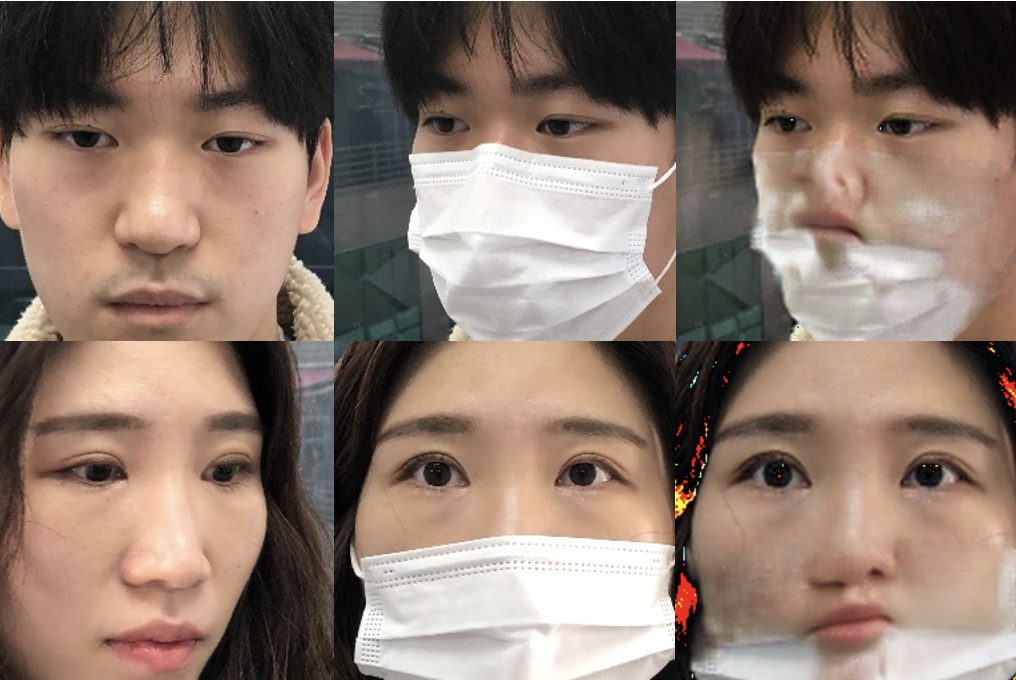
\includegraphics[width=0.8\linewidth]{images/bad-results.png}
  \caption{\emph{Failure cases of our model.} Generated images from actual real-life masked images.
  Starting from the left are: the identity image, masked image, and the generated output.}
  \Description{Image results}
  \label{images:bad-results}
\end{figure}


To alleviate this problem, we believe that in future works, by implementing a process of generating masked images within the model framework (similar to CycleGAN \cite{CycleGAN}), then the masked images may follow the real-world data distribution. Also, using a more diverse dataset like CelebA \cite{CelebA} or FFHQ \cite{StyleGAN} can help with this problem as well.

Another problem is that noise-like artifacts appeared in the generated images. We have mostly solved this problem by normalizing the output to the PSP encoder. However certain results still show these artifacts (Figure \ref{images:noise-artifact}).
We currently suspect this 

\begin{figure}[ht]
  \centering
  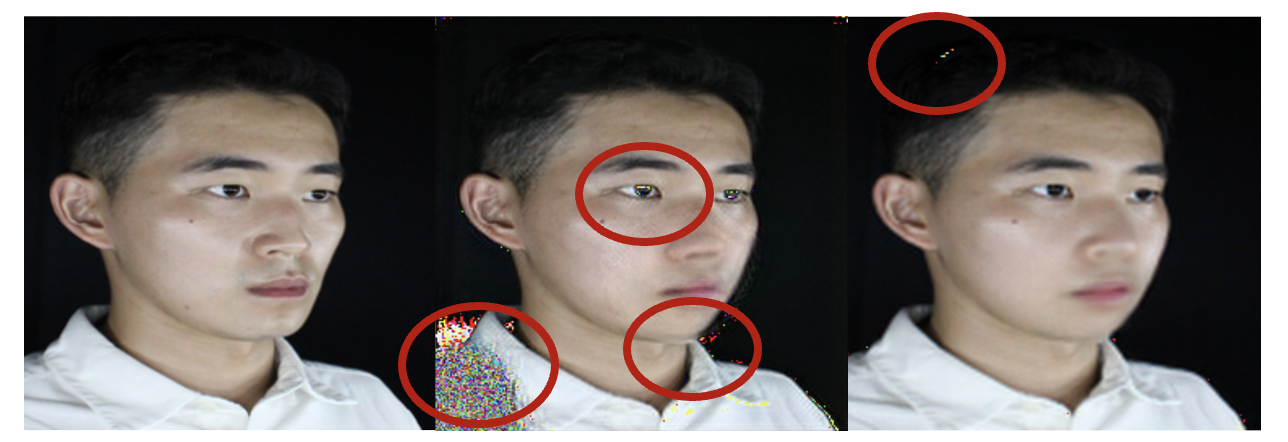
\includegraphics[width=0.8\linewidth]{images/noise-artifacts.png}
  \caption{\emph{Noise artifacts in the images.} Although the problem of large noise-like artifacts are greatly reduced, generated images still contain these artifacts.
  Starting from the left are: the ground truth, results with the unnormalized identity features, and our final model.}
  \Description{Image results}
  \label{images:noise-artifact}
\end{figure}

Finally, while our generated images show higher quality than most other projects, our results
still present mild blurriness and misrepresented facial attributes. We believe this is because
of the high L1 loss \cite{Image-Restoration-Loss}, however our experiment results show that low L1 loss does not lead to optimal results. This may be correlated to our changed architecture, however further insight is required to know the exact reasons and method for improvement.

Other improvements can be done to our model, such as encoding additional information such as emotion as a condition. There are also other methods of identity extraction \cite{PersonalDiffusion} that could give higher performance.

\subsection{Other Tasks}
We believe our proposed network can be expanded to tasks other than mask removal. Our model has
the advantage of doing image-to-image translation while adding additional information as a form of
an image. This has many use cases, especially in the case of personalized image generation, where a user might attempt to translate an image while having the identity information intact. Facial reconstruction, image inpainting could all be one of many examples where our proposed architecture can be used.

\section{Conclusion}
We introduced a novel neural network architecture for personalized image-to-image translation by
focusing on removing face masks. Our network has achieved considerable quality generation compared
to other baseline models and even generating under extreme conditions, all while retaining the
source identity with high accuracy. This network is very fast and can be expanded to other tasks
and is also applicable to real-world use cases.

\bibliographystyle{ACM-Reference-Format}
\bibliography{citations}

\end{document}
\endinput
